% To produce pdf under linux, run
% pdflatex hw3.tex 

\documentclass{article}
\usepackage{amsmath,amssymb}
\usepackage{bbm}
\usepackage{graphicx}
\usepackage{url}
\usepackage{hyperref}
\usepackage{color}

\def\bfx{\mathbf x}
\def\R{\mathbb R}
\def\E{\mathbb E}
\def\argmax{\mathrm{argmax}}

\title{CS761 Spring 2017 Homework 3}
\author{Assigned Apr. 6, due Apr. 20} 
\date{}
\begin{document}
\maketitle

Instructions: 
\begin{itemize}
\item Homeworks are to be done individually.
\item Typeset your homework in latex using this file as template (e.g. use pdflatex).  Show your derivations.
\item Hand in the compiled pdf (not the latex file) online.  Instructions will be provided.  We do not accept hand-written homeworks.  
\item Homework will no longer be accepted once the lecture starts.
\item Fill in your name and email below.  
\end{itemize}

%%%%%%%%%%%%%%%%%%%%%%%%%%%%%%%%%%%%%%%%%%%%%%%%%%%%%%%%%%%%%%%%%%%%%%%%%
% Insert your name and email here:

Name:                      

Email: 

\newpage % Please keep this page-break
% Do not include any identifying information below this line.
%%%%%%%%%%%%%%%%%%%%%%%%%%%%%%%%%%%%%%%%%%%%%%%%%%%%%%%%%%%%%%%%%%%%%%%%%

(4 questions, 25 points each)

\begin{enumerate}


\item 
The Wisconsin State Climatology Office keeps a record on 
the number of days Lake Mendota was covered by ice at
\url{http://www.aos.wisc.edu/~sco/lakes/Mendota-ice.html}.
The article DETERMINING THE ICE COVER ON MADISON LAKES at
\url{http://www.aos.wisc.edu/~sco/lakes/msn-lakes_instruc.html}
serves as a fine example of the Wisconsin tradition to integrate science with beer.

\begin{enumerate}
\item
As with any real problems, the data is not as clean nor as organized as one would like for machine learning.
Produce a clean data set starting from 1855-56 and ending in 2016-17 for the output variable DAYS.
You do not need to attach your data set, but please produce a scatter plot of year vs. DAYs.
Show us the sample mean and sample variance (round to 5 digits after decimal point).

\hspace*{-4cm}  
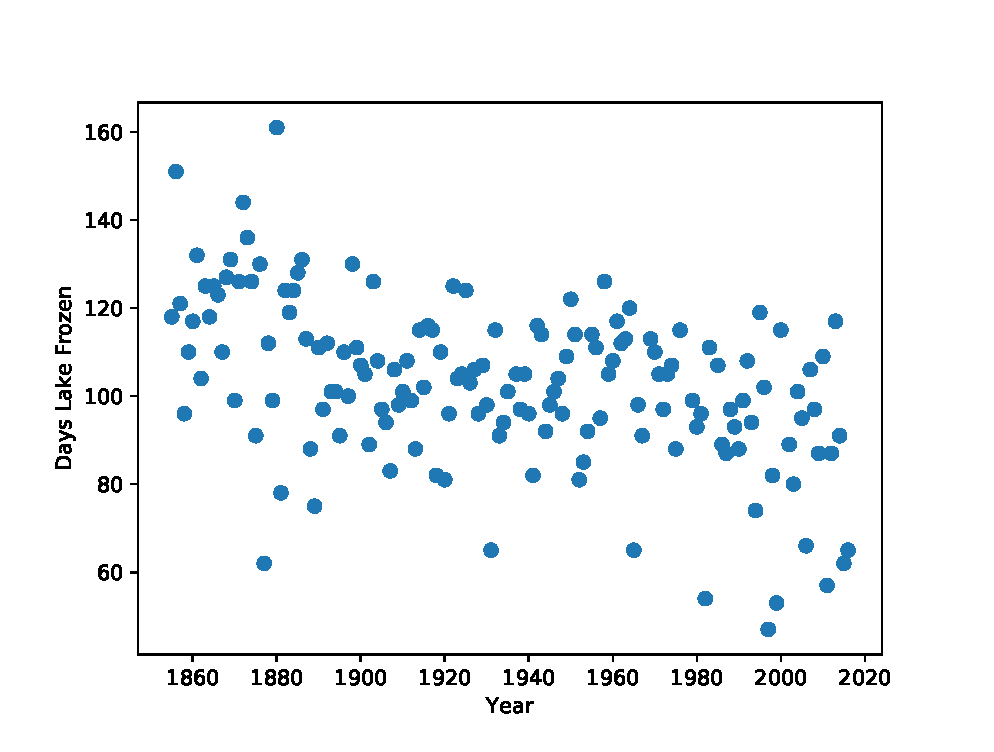
\includegraphics[scale=1]{ice_scatter}

\color{red}
\textbf{Mean:} = 102.80769  
\textbf{Variance:} = 343.57840
\color{black}
\item 
Perform ordinary least squares to estimate a linear model 
$$y = \alpha + \beta x$$
where $y$ is DAYS and $x$ is the year.
For example, for 1855-56 the year is 1855.
Show us $\hat{\alpha}, \hat{\beta}$, and an estimate of the standard error on $\beta$: $\widehat{s.e}(\hat{\beta})$.

\color{red}
$$
\hat{\beta} = -0.18561 \qquad \hat{\alpha}= 461.78577  \qquad \hat{s.e}\{\hat\beta\} = \sqrt{s^2 (X^\top X)^{-1} } = 0.00068
$$
\color{black}

\item
Perform nonparametric kernel regression using the Nadaraya-Watson estimator on this data set (input: year, output: days).
Use the Gaussian kernel.
Write your own code for the Nadaraya-Watson estimator.
Show us the leave-one-out score (Equation 23 in lecture notes \url{http://pages.cs.wisc.edu/~jerryzhu/cs761/kde.pdf}) for bandwidth 
$h=10^{-1}, 10^{-0.9}, 10^{-0.8}, \ldots, 10^2$, respectively.

\color{red}
\begin{verbatim}
h = 10^-1, LeaveOneOut Score = NaN
h = 10^-0.9, LeaveOneOut Score = 470.15966
h = 10^-0.8, LeaveOneOut Score = 472.28524
h = 10^-0.7, LeaveOneOut Score = 472.28526
h = 10^-0.6, LeaveOneOut Score = 472.28526
h = 10^-0.5, LeaveOneOut Score = 472.28511
h = 10^-0.4, LeaveOneOut Score = 472.24836
h = 10^-0.3, LeaveOneOut Score = 471.07843
h = 10^-0.2, LeaveOneOut Score = 461.79288
h = 10^-0.1, LeaveOneOut Score = 435.06801
h = 10^0, LeaveOneOut Score = 398.43935
h = 10^0.1, LeaveOneOut Score = 366.57279
h = 10^0.2, LeaveOneOut Score = 343.70665
h = 10^0.3, LeaveOneOut Score = 327.49724
h = 10^0.4, LeaveOneOut Score = 315.25907
h = 10^0.5, LeaveOneOut Score = 305.71688
h = 10^0.6, LeaveOneOut Score = 298.58151
h = 10^0.7, LeaveOneOut Score = 292.96769
h = 10^0.8, LeaveOneOut Score = 287.56533
h = 10^0.9, LeaveOneOut Score = 282.08339
h = 10^1, LeaveOneOut Score = 277.3443
h = 10^1.1, LeaveOneOut Score = 274.17402
h = 10^1.2, LeaveOneOut Score = 272.96093
h = 10^1.3, LeaveOneOut Score = 273.91815
h = 10^1.4, LeaveOneOut Score = 277.05608
h = 10^1.5, LeaveOneOut Score = 281.81211
h = 10^1.6, LeaveOneOut Score = 287.40215
h = 10^1.7, LeaveOneOut Score = 294.11911
h = 10^1.8, LeaveOneOut Score = 302.82929
h = 10^1.9, LeaveOneOut Score = 312.90299
\end{verbatim}
\color{black}
 
\item
For $h=10^{-1}, 10^{2}$ and the optimal $h$ you found, respectively,
plot the function estimated by Nadaraya-Watson.
\end{enumerate}


\item 
Consider a Gaussian Process $f \sim GP(m,k)$ over $\R$ with mean function
$$m(x) = \sin(\frac{\pi x}{100}) + \frac{x}{100}$$
and kernel function
$$k(x,x') = \frac{1}{16}\exp\left( -\frac{(x-x')^2}{2\sigma^2} \right).$$
\begin{enumerate}
\item
Let $\sigma=40$ (note: this is the standard deviation, not variance).  Approximate the random function $f$ by drawing $f(1), f(2), \ldots, f(100)$ from the appropriate marginal distribution.  Plot the curve by connecting the dots.
Show six such random functions on the same plot, together with the mean function $m$.
\item Do the same with $\sigma=10$.
\item Do the same with $\sigma=1$.
\item
Let $\sigma=40$.
Now let us observe $f(40)=0$ and $f(120)=1$.
Now draw $f$ from the posterior Gaussian Process conditioned on these two observations.
Again, show six such $f$ from the posterior on the same plot.

\item Do the same with $\sigma=10$.
\item Do the same with $\sigma=1$.
\end{enumerate}


\item 
Imagine a stick of length $a$.  On the ground, draw parallel lines $a$ apart.
Randomly throw the stick to the ground.
Each time, the stick may or may not intersect with a line.
\begin{enumerate}
\item What is the probability that the stick intersects with a line?  Show your work.
\item Propose a Monte Carlo method for estimating $\pi$ based on this.  
\item Actually perform the experiment.  Tell us about it.
\end{enumerate}

\item 
Consider an undirected graphical model on a binary tree with 15 nodes.
Each node takes value in $\{-1,1\}$.
All edges share the same potential function $\psi(u,v) = \exp(\alpha u v)$, where $u,v$ are a pair of parent-child nodes.

  \begin{enumerate}
  \item Write down the joint probability distribution defined by this graphical model.
  \item Let $\alpha=1$.  Let $r$ be the root node and $s$ be the left-most leaf node.
  Use brute force (enumerating all trees) to compute $p(r \mid s=1)$.
  \item Implement Gibbs sampling to estimate $p(r \mid s=1)$.  Start with the all-minus-1 tree except for $s=1$.  Go over levels in top-down order, left-to-right within each level.
  Discard a burn-in of $10^4$ samples.  Use the next $10^5$ samples for estimation.  Do not perform thinning.
  \item Implement Metropolis-Hastings sampling to estimate $p(r \mid s=1)$.  Clearly define and discuss your proposal distribution (which has to be different than Gibbs).  Use the same burn-in and number of samples as above.
  \end{enumerate}



\end{enumerate}
\end{document}
